\section{Problem Analysis}\label{sec:problem-analsysis}

	The project solution can be divided in the structure showed in Figure \ref{fig:projectProblem}.
	
	\begin{figure}[htbp]
		\centering
			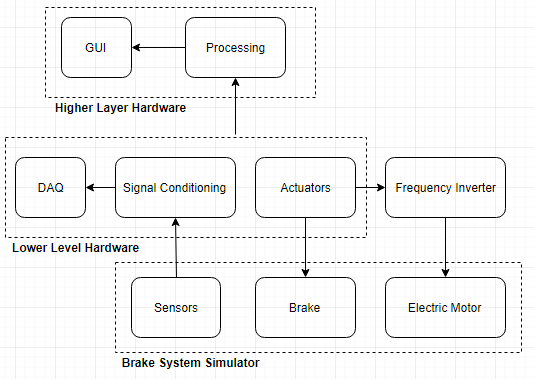
\includegraphics[scale=0.9]{figuras/fig-projectProblem}
		\caption{Project Problem Depuration}
		\label{fig:projectProblem}
	\end{figure}
	

	\subsection{Brake System Simulator}\label{ssec:brakeSystemSimulator}
		
		The \textit{Brake System Simulator} block as the name says comprehends the hardware responsible for simulating the environment of a brake system, the two basic components are the \textbf{Brake} component itself (in this case being a disc brake system and peripherals) and a \textbf{Electric Motor} to accelerate the rotor in order to simulate the speed a vehicle wheel might be submitted. A \textbf{Transducers/Sensors} block was also added, without acquiring a physical/mechanical quantities such as temperature and pressure, a brake test would be useless because no possible technical analysis could be done afterwards. The \textbf{Transducers/Sensors} block was placed inside the \textit{Brake System Simulator} block because the sensors and transducers will be placed arround the components of this major block.

	\subsection{Higher Layer Hardware}\label{ssec:higherLayerlHardware}
	
		This layer needs to do all the heavy data processing, \textit{i.e.}, converting and dealing with the information that flows through all the structure. The \textit{GUI} block is the one responsible for acquiring and displaying computer information in a human-friendly format. Although developing this part of the solution is not part of this thesys it it important to understand its importance.

	\subsection{Lower Layer Hardware}\label{ssec:lowerLayerlHardware}

		This layer of hardware will make the translation from physical/mechanical quantities to computer data and \textit{vice versa}, \textit{i.e.}, converting physical/mechanical quantities to voltage and than to bytes of information and also on the opposite way (bytes to voltage and voltage to physical/mechanical quantities). Tranducers signals are not always ready to read, as mentioned in Section \ref{ssec:instrumentation-amplifier}, Instrumentation Engineering also involves doing Signal Conditioning to amplify and filter this signals. Controlling the system also involves designing circuits to generate the desired digital and analog output channels.
		\par
		Based on the matters analysed on the previous sections of this paper a hardware architecture was defined and it displayed on the following Figure \ref{fig:hardwareProject}.
	
		\begin{figure}[htbp]
			\centering
			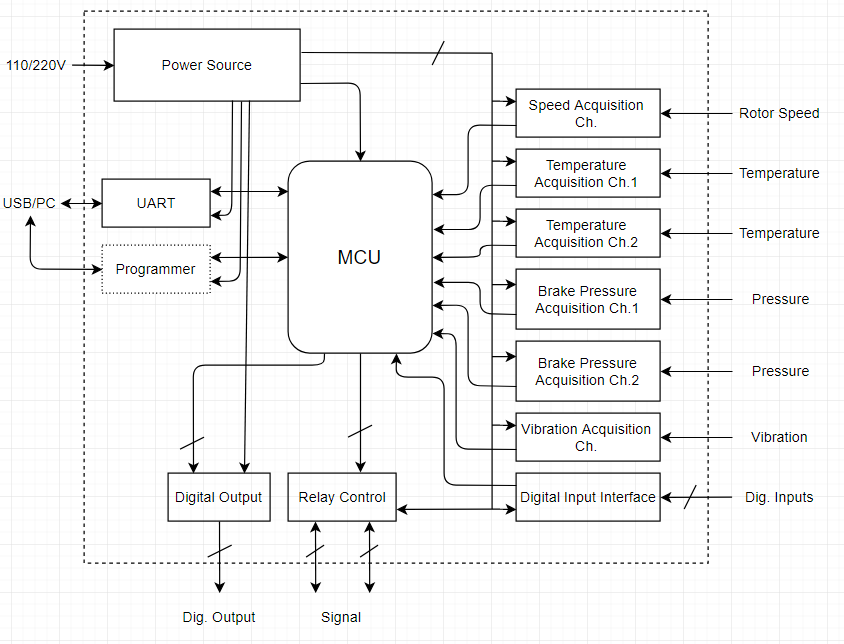
\includegraphics[scale=0.8]{figuras/fig-hardwareProject}
			\caption{Hardware Project Architecture \cite{hw-proj}}
			\label{fig:hardwareProject}
		\end{figure}

		It is possible to see that each type of transducer will have a specific circuit in order to perform signal conditioning as better as possible according to the type of transducer parameters. Also it is possible to observe that there will be special circuits to interface the MCU with digital outputs and inputs alongside with analog outputs. Regarding the analog outputs, it is also interesting to have a feedback path to the MCU so adjustments can be made in order to guarantee that the analog outputs voltages are correct according to the desired quantities. Moreover, a power supply block should be designed to generate a stabilized voltage to power up all the circuit modules. Last but not least, a communication port (USB) was placed, through this port the communication with the upper layer of hardware will be done.

		\subsubsection{Lower Level Hardware Interfaces}\label{sssec:lower-level-hardware-interfaces}

			Based on the previous considerations and considering possible future usages for the designed product, this are the following hardware interfaces.

			\begin{itemize}
				\item \textit{Sensor Inputs:}
					\begin{itemize}
						\item Speed Sensor.
						\item Temperature Sensor 1.
						\item Temperature Sensor 2.
						\item Brake Force Sensor 1.
						\item Brake Force Sensor 2.
						\item Vibration Sensor 1.
					\end{itemize}
				\item \textit{Digital Interfaces:}
					\begin{itemize}
						\item Output 1.
						\item Output 2.
						\item Output 3.
						\item Input 1.
						\item Input 2.
						\item Input 3.
					\end{itemize}
				\item \textit{Analog Outputs:}
					\begin{itemize}
						\item Output 1.
						\item Output 2.
					\end{itemize}
				\item \textit{Communication Ports:}
					\begin{itemize}
						\item USB Port 1.
					\end{itemize}
			\end{itemize}